\section{What Flips: The Cross-Space Sign Reversal}
\label{sec:crossspace}

%% ---------------------------------------------------------------
%% Cluster: the sign-flip and its consequences. The page-1 concept
%% figure (\cref{fig:signflip}) is defined in sec_v3/0_abstract.tex;
%% the hero exhibit of THIS cluster is the full-width portability
%% heatmap fig:portability, floated at the top.
%% ---------------------------------------------------------------

\begin{findingframe}
\textbf{The portability failure, in brief} (\cref{fig:portability}). A single
zero-cost proxy reverses the sign of its relationship to quality when moved
between two axes of the same benchmark. Three within-NB201 examples motivate the
analysis; $9/13$ proxies reverse descriptively somewhere in the broader map and
four cross-benchmark cases meet the strict support rule. The \px{cond-sum}
failure is dimension-linked, and two named budget-search traps cost $+5.40$ and
$+1.97$ accuracy points at $K{=}10$, while two null directions cost zero.
\end{findingframe}

\noindent We summarize above and elaborate next.

%-------------------------------------------------------------------------
% HERO EXHIBIT: 13x7 cross-space portability heatmap (full-width figure*).
%-------------------------------------------------------------------------
\begin{figure*}[t]
  \centering
  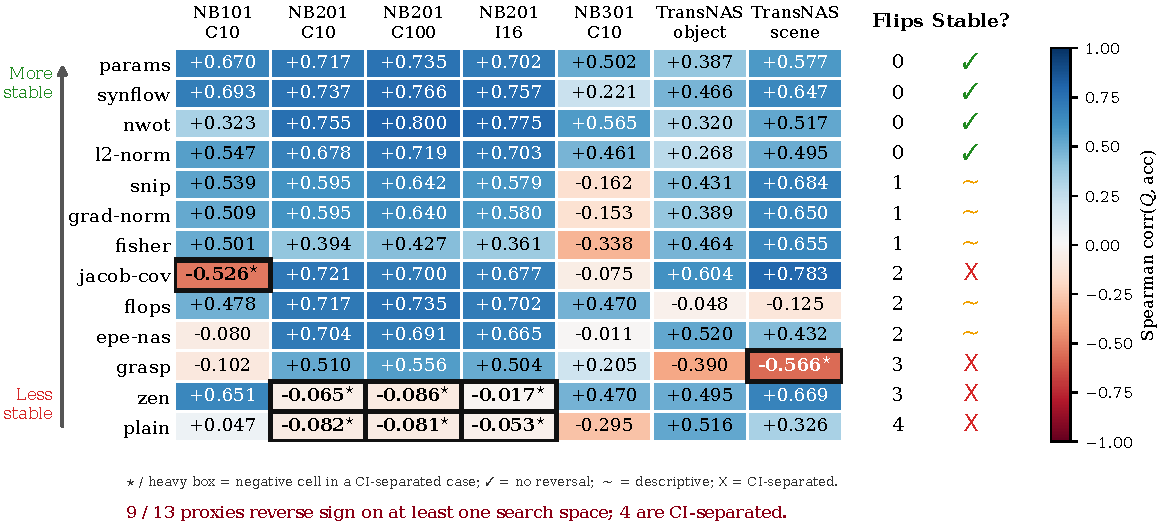
\includegraphics[width=\textwidth]{figures/fig4_portability_full.pdf}
  \caption{\textbf{Cross-space portability matrix.} Spearman
  $\corr(Q,\acc)$ for $13$ standard proxies over $7$ search spaces, with rows
  ordered most-to-least stable (flip count ascending, then mean $|\rho|$).
  Heavy boxes and $\star$ mark negative cells in the four CI-separated cases
  (\px{jacob-cov}, \px{grasp}, \px{zen}, \px{plain}); the side panel reports
  each proxy's flip count and stability tier ($\checkmark$: no reversal;
  $\sim$: descriptive reversal; $\mathsf{X}$: CI-separated reversal). Nine of $13$ proxies
  reverse descriptively on at least one space, while four meet the strict rule.
  Per-space sample sizes and intervals are in \cref{tab:app-portability} and
  \cref{app:generalize-evidence}.}
  \label{fig:portability}
\end{figure*}

\noindent\textbf{The cleanest instance lives \emph{inside} a single benchmark.}
The preceding analysis (\cref{sec:cap-train}) found a capacity-associated factor
that recurs on both axes
and a trainability residual that is statistically distinct and partly accessible. We
now ask whether a single proxy carries the same signal once it is moved to a
structurally different axis. NB201's two one-knob axes (\cref{sec:setup}) let a
reversal be read off without blaming a change of dataset, recipe, or proxy
implementation. We therefore center the orientation-free accuracy correlation
$\corr(Q,\acc)$ and treat the per-proxy trainability partial
$\partialcorr(Q,T\mid\erank,\params)$ as an orientation-sensitive secondary view.

%-------------------------------------------------------------------------
\noindent\textbf{The sign-flip.}\label{sec:result4}\label{sec:r4}\label{sec:signflip}\label{find:flip}{}
The cleanest, orientation-free result is the raw accuracy-slot flip: a single
proxy's correlation with quality reverses from positive on the topology
(TSS) axis of NAS-Bench-201 to negative on the size (SSS) axis, with no
sign-orientation rule applied. The spectral conditioning functionals make this
plain: \px{cond-sum} goes $+0.88\,{\to}\,-0.77$ ($n{=}324/138$),
\px{meco} $+0.88\,{\to}\,-0.79$, and \px{grasp} $+0.55\,{\to}\,-0.19$, the page-1
headline (\cref{fig:signflip}). The spectral arm also clears a faithfulness
check: the TSS value is consistent with Dextr's published $\sim\!0.88$
(\px{cond-sum} = the official inverse-condition statistic, $0$ hook exceptions;
\cref{app:faithfulness}), making a simple TSS implementation mismatch less
plausible. A
reversal this large in the raw, un-oriented accuracy slot is the central flip we
analyze.

\noindent Under per-axis outcome-informed orientation, the same reversal also reaches the trainability partial
$\partialcorr(Q,T\mid\erank,\params)$, the very slot previewed in
\cref{fig:results}(b), though here the evidence is more graded. The CI-separated
trainability-slot reversals across both axes are carried by \px{meco}
($+0.291\,{\to}\,-0.398$) and \px{Q-adapt-rot} ($+0.143\,{\to}\,-0.602$); the
headline \px{cond-sum} SSS trainability partial is $-0.141$ with $95\%$ CI
$[-0.31,+0.04]$, which spans zero, so it is consistent-with rather than a
CI-separated trainability-slot flip, as are the SSS partials for \px{jacob-cov}
and \px{gradsign} (\cref{app:perproxy-signflip}, \cref{tab:app-perproxy}).\linebreak One
caveat is decisive: because each proxy was sign-oriented per axis by its own
accuracy correlation, the trainability-slot direction is entangled with the
outcome-informed rule. In the global-orientation control, PCA variance and
score/capacity association are unchanged but loading agreement drops from
$0.869$ to $0.461$; \px{meco}'s SSS partial also changes orientation. We therefore
treat these trainability-slot directions as orientation-sensitive exploratory
evidence, not as an independent cross-axis flip. The raw accuracy-slot reversals
above remain orientation-free.

%-------------------------------------------------------------------------
\noindent\textbf{The outcome-informed orientation's narrow survivor.}\label{sec:mechanism}\label{find:ntk}\label{find:mech}{}
Under per-axis outcome-informed orientation, one proxy---\px{ntk}---has a \emph{trainability partial}
$\partialcorr(Q,T\mid\erank,\params)$ that is positive with a CI excluding zero on
both axes ($+0.180$ TSS / $+0.241$ SSS); its $T_{\mathrm{slope}}$ partial also
survives BH-FDR on both axes. The qualifier matters: \px{ntk} survives
\emph{in this trainability-partial slot at the full-zoo sample}, not as a portable
accuracy predictor---as a raw accuracy ranker it is anti-correlated on \emph{both}
axes (\cref{tab:app-perproxy}). This is not an orientation-robust uniqueness
claim: under the globally fixed rule both \px{meco} and \px{ntk} have positive
marginal intervals on both axes, an exploratory, unadjusted comparison. At the
larger standard-proxy base \px{synflow} and \px{zico} also join \px{ntk} under
this rule; per-proxy cells are in \cref{app:mechanism-evidence}.

\noindent\textbf{The \px{cond-sum} failure is dimension-linked, not an identified
mechanism.} On balanced $n{=}500/500$ cohorts, the raw correlation is
$+0.887/-0.781$ (TSS/SSS). Dividing by cached spectrum length gives
$+0.842/-0.785$, and dividing by effective rank gives $+0.418/-0.885$.
Within SSS, however, the partial of the raw score is only $-0.079$ after
effective-rank control and $-0.068$ after joint cached-length, effective-rank,
and parameter controls. Exact cached-length matching is not identifiable because
the supports do not overlap (TSS $142$--$502$; SSS $118$--$122$). An unmatched
effective-rank common-range sensitivity yields $-0.318/-0.885$, removing the
cross-axis sign difference, but only 103 TSS records fall in that range. Finally,
the cached count is not a validated representation dimension. These results
support a dimension-linked/proxy-geometry-dependent transport failure. An exact
representation-dimension-matched test cannot be performed because that field is
absent from the available artifacts.

%-------------------------------------------------------------------------
\begin{table}[H]
\centering\small\setlength{\tabcolsep}{5pt}
\begin{tabular}{lrr}
\toprule
Score correlation ($n{=}500$ per axis) & TSS & SSS\\
\midrule
\px{cond-sum} (raw) & $+0.887$ & $\mathbf{-0.781}$\\
\px{cond-sum}/cached length & $+0.842$ & $\mathbf{-0.785}$\\
\px{cond-sum}/effective rank & $+0.418$ & $\mathbf{-0.885}$\\
$R_{\alpha=1}$ (effective rank, NEAR) & $+0.864$ & $+0.911$\\
\bottomrule
\end{tabular}
\caption{\textbf{Cached normalizations do not by themselves remove the
full-population flip.} Effective-rank partial/common-range sensitivities and the
non-overlapping cached-length support require the narrower dimension-linked
interpretation in the text.}
\label{tab:spectral-body}
\end{table}

\noindent Full normalization intervals, within-length strata, the common-range
sensitivity, and the reason exact dimension matching is unavailable are in
\cref{app:r2-dimension}.

\noindent\textbf{It partly generalizes.}\label{sec:generalize}\label{find:generalize}{}
Of the $9$ proxies that reverse the sign of $\corr(Q,\acc)$ on at least one of the
seven columns, exactly four survive a strict test---two columns whose
$2000$-resample $95\%$ intervals are disjoint, each individually FDR-significant---and
they fall into two magnitude tiers (\cref{fig:portability}). Two are large
bilateral flips: \px{jacob-cov} ($+0.78$ TransNAS-scene vs.\ $-0.53$ NB101) and
\px{grasp} ($+0.56$ NB201-CIFAR-100 vs.\ $-0.57$ TransNAS-scene). The other two are
attenuations-to-near-zero rather than full reversals: \px{zen} ($+0.67$ vs.\
$-0.086$) and \px{plain} ($+0.33$ vs.\ $-0.082$), whose negative side is significant
only by the large NB201 sample. The remaining candidates fail the bar---small-$n$
NB301 attenuations, \px{epe-nas}'s lone NB101 cell, and \px{flops}'s near-zero TransNAS
reversal---and only NB301 stays excluded as degenerate
(\cref{app:generalize-evidence}). This cross-space arm reintroduces the dataset and
sample-size confounds the within-NB201 design removed, so these four flips are
weaker evidence than the within-benchmark reversal. The decomposition behind this
also replicates across NB201's three datasets---capacity stays the leading term and
trainability a comparable contributor (\cref{tab:decomp-body})---while the deep
capacity/trainability decomposition itself remains NB201-only. Full per-space
values and CIs are in \cref{app:generalize-evidence},
\cref{tab:app-portability,tab:app-spectral}, and \cref{app:crossspace}.

\noindent\textbf{Recent controls bound the claim.}
SWAP~\cite{peng2024swap} is positive on TSS/SSS ($0.798/0.778$), as is
AZ-NAS~\cite{aznas2024} ($0.922/0.740$),
with architecture-bootstrap intervals excluding zero. Thus SWAP is one
sign-stable recent control, not evidence about every recent proxy;
L-SWAG~\cite{casarin2025lswag}/InTrain~\cite{intrain2026}
remain unevaluated because no official, licensed, auditable implementation was
available as of August 25, 2026 (intervals and protocol in
\cref{app:r2-recent}).

\noindent\textbf{The full decomposition remains NB201-only.}
Across 49,674 audited external records, official artifacts expose only 13 finite
proxy fields and lack the complete aligned proxy/capacity/training field classes
required by \cref{eq:decomp}. No population jointly has sufficient proxy
coverage, effective rank, exact early $T$, and final accuracy, so
\cref{eq:decomp} has zero eligible external rows. We report the missing-field
coverage instead of constructing a surrogate, while retaining the raw map beyond
NB201 (audit in \cref{app:r2-external}).

%-------------------------------------------------------------------------
\noindent\textbf{The flip has a search cost.}\label{sec:searchtransfer}\label{find:searchtransfer}{}
The reversal changes which architecture a budget-$K$ search returns. The baseline
transfers the single best-on-source proxy as-is; the sign-stability screen uses a
target-CALIB split to reject a proxy whose orientation does not transport, then
scores a disjoint target-EVAL split. No network is trained, but cached target
accuracy is used for calibration. On the TSS${\to}$SSS trap, the gap to
the source-best proxy is $+7.83/+6.62/+5.40/+3.00$ at $K{=}1/5/10/50$.
The scene${\to}$NB101 trap gives $+1.11/+1.55/+1.97/+1.56$; the reverse
SSS${\to}$TSS and scene${\to}$NB201 nulls are zero at every budget. At the
pre-specified moderate budget $K{=}10$, percentile intervals under the
target-position resampling protocol are
$[4.386,6.435]$ and $[0.626,3.133]$ for the two traps
(\cref{tab:searchtransfer}). All $K{=}1/5/10/50$ results are retained to avoid
favorable-budget selection. These are named trap costs, not average gains.

%-------------------------------------------------------------------------
\noindent\textbf{The diagnostic is target-calibrated, not fully label-free.}{}
The CALIB and EVAL positions are disjoint under the target-position
resampling protocol, but
canonical architecture identities can overlap. A second protocol partitions
identities first and has zero CALIB/EVAL identity overlap; its K=10 intervals are
$[5.057,5.599]$ and $[1.487,2.208]$, with both nulls still zero. The protocols
use different resampling units and are reported separately. The evaluation
also includes params, SynFlow, fixed rank-ensemble, random, negative, and
unfavorable comparisons. The screen is useful for the two evaluated trap
directions, but
does not dominate every baseline and is not a universal NAS remedy.
Full budget results, baseline comparisons, and the identity-disjoint sensitivity
are reported in Supplementary Sec.~\ref{app:r2-search}
(\emph{Search consequence and sensitivity protocols}).

\begin{table}[htbp]
  \centering
  \small
  \caption{\textbf{K=10 search consequence} (cached accuracy, no training).
  Values are target-CALIB screen minus transported source-best proxy; intervals
  are non-inferential percentile summaries under the target-position
  resampling protocol.}
  \label{tab:searchtransfer}
  \begin{tabular}{@{}lrc@{}}
    \toprule
    Direction & gap (pts) & percentile interval \\
    \midrule
    TSS${\to}$SSS (trap) & $+5.402$ & $[4.386,6.435]$ \\
    SSS${\to}$TSS (null) & $0.00$ & $[0,0]$ \\
    scene${\to}$NB101 (trap) & $+1.973$ & $[0.626,3.133]$ \\
    scene${\to}$NB201 (null) & $0.00$ & $[0,0]$ \\
    \bottomrule
  \end{tabular}
\end{table}

\paragraph{Multiple-comparison control.}
The strict cases do not rely only on unadjusted screening: $34$ of the $58$
per-proxy partial cells and $78$ of the $91$ portability cells survive BH-FDR,
and each of the four CI-separated
flips is individually FDR-significant; the full accounting is in \cref{tab:app-fdr}
(\cref{app:generalize-evidence}).
